\section{Proposed Method}
\label{sec:method}

% Overview of the proposed quality-aware measurement (M3). Drawn in TikZ so it is editable.
\begin{figure*}[t]
\centering
\resizebox{\textwidth}{!}{%
\begin{tikzpicture}[
  font=\sffamily\small, >=Stealth,
  box/.style={draw=black!55, rounded corners=2pt, fill=#1, align=center, inner sep=4pt,
              minimum height=1.0cm, text width=2.35cm},
  box/.default=white,
  arr/.style={->, thick, black!65},
  lab/.style={font=\sffamily\scriptsize, text=black!65, align=center}
]
% column 1: input
\node[box=black!4] (in) at (0,0) {Input photo $I$\\[-1pt]\scriptsize (single 2D image)};
% column 2: two detections
\node[box=blue!8]  (d1) at (3.3, 0.9) {Face Landmarker\\on $I$ $\rightarrow L$};
\node[box=blue!8]  (d2) at (3.3,-0.9) {Face Landmarker\\on $\mathrm{flip}(I)$};
% column 3: mirror test
\node[box=blue!15, text width=2.9cm] (mt) at (6.9,-0.9) {\textbf{Mirror test}\\[-1pt]\scriptsize unflip $x\!\mapsto\!W\!-\!x$, re-index by\\[-2pt]\scriptsize canonical mirror map $\pi$ $\rightarrow U$};
\node[box=blue!15, text width=2.9cm] (avg) at (6.9, 0.9) {$\bar L=\tfrac12(L+U)$\\[-1pt]\scriptsize $\delta=\overline{\|L-U\|}/\mathrm{IOD}$};
% column 4: 68 mapping + axis
\node[box=green!10, text width=2.7cm] (map) at (10.4, 0.9) {478$\rightarrow$68 map\\[-1pt]\scriptsize mirror-consistent,\\[-2pt]\scriptsize fitted on train split};
\node[box=green!10, text width=2.7cm] (ax) at (10.4,-0.9) {\textbf{Fitted symmetry axis}\\[-1pt]\scriptsize $\min_{\theta,\rho}\sum_i\|\mathcal R_{\theta\rho}(p_{\pi(i)})-p_i\|^2$};
% column 5: measures
\node[box=green!18, text width=2.6cm] (meas) at (13.8,-0.9) {Global $A$, regional $A_r$\\[-1pt]\scriptsize $a_i=\|r_i\|/(2\,\mathrm{IOD})$};
% gate
\node[box=orange!18, text width=2.6cm] (gate) at (13.8, 0.9) {\textbf{Quality gate}\\[-1pt]\scriptsize size, sharpness, exposure,\\[-2pt]\scriptsize $|$yaw$|$, $|$pitch$|$, $\delta$, $\delta_r$};
% output
\node[box=black!6, text width=2.8cm] (out) at (17.3,0) {\textbf{Output}\\[-1pt]\scriptsize accept / caution / reject,\\[-2pt]\scriptsize $A\pm|A(L)-A(U)|$,\\[-2pt]\scriptsize reliable regions only};

\draw[arr] (in.east) -- ++(0.35,0) |- (d1.west);
\draw[arr] (in.east) -- ++(0.35,0) |- (d2.west);
\draw[arr] (d2) -- (mt);
\draw[arr] (d1.east) -- (avg.west);
\draw[arr] (mt) -- (avg);
\draw[arr] (avg) -- (map);
\draw[arr] (map) -- (ax);
\draw[arr] (ax) -- (meas);
\draw[arr] (avg.north) -- ++(0,0.45) -| node[lab, pos=0.25, above]{$\delta$, per-region $\delta_r$} (gate.north);
\draw[arr] (d1.north) -- ++(0,0.75) -| node[lab, pos=0.27, above]{pose (transformation matrix), face crop statistics} ([xshift=6mm]gate.north);
\draw[arr] (gate.east) -- ++(0.3,0) |- ([yshift=2mm]out.west);
\draw[arr] (meas.east) -- ++(0.3,0) |- ([yshift=-2mm]out.west);
\end{tikzpicture}}
\caption{\textbf{Overview of the proposed quality-aware measurement (variant M3).}
The landmarker is run on the photo and on its mirror image. Because a horizontal flip only
swaps anatomical sides, an ideal detector returns the same geometry twice; the disagreement
$\delta$ is a ground-truth-free check of landmark reliability, and the average $\bar L$
cancels any left/right bias of the detector. Asymmetry is measured on the standard 68-point
layout with fixed anatomical pairs and a fitted (not assumed) symmetry axis, and a score is
only reported when the quality/pose gate does not reject the image.}
\label{fig:overview}
\end{figure*}


\Cref{fig:overview} shows the pipeline. Each step is described below, together with the
reason it is there.

\subsection{Landmarks and fixed bilateral correspondence}
\label{sec:corr}
\textbf{Detection.} We use the MediaPipe Face Landmarker (Tasks API, float16 model) in
image mode. It returns $L\in\mathbb{R}^{478\times2}$ in pixels and a $4{\times}4$
canonical-to-camera transformation matrix, from which we read yaw, pitch and roll (ZYX
Euler angles). \emph{Why:} it runs on CPU in real time, needs no training, and its mesh has
a \emph{fixed topology}, which makes anatomical correspondence possible.

\textbf{Mirror permutation $\pi$.} MediaPipe's canonical face model is exactly
left--right symmetric. Reflecting it ($x\!\mapsto\!-x$) and taking the nearest vertex
gives an involution $\pi$ on the 468 face vertices, with a maximum residual of $0$:
220 bilateral pairs and 28 midline vertices (iris points are paired explicitly). A
vertex is therefore always compared with its own anatomical twin.
\emph{Why not KD-tree matching:} prior tools~\cite{nashokan_facialasymmetry,
varghaei2025aesthetic} reflect each left-side vertex and take the \emph{nearest} right-side
vertex. In a dense mesh the nearest vertex is often a neighbour of the true twin, so the
matching absorbs part of the asymmetry it should measure. On LFPW, \kdWrong\% of KD-tree
matches are not the anatomical partner (\cref{fig:corr}).

\textbf{478$\to$68 mapping.} We report on the 300-W 68-point layout, whose bilateral pairs
are defined by the annotation protocol and for which expert annotations exist. For each
iBUG point $k$ and mesh vertex $v$ we compute $E_{kv}$, the median over the 810
\emph{training} images of $\|L_v-G_k\|/\mathrm{IOD}$, and choose, for each iBUG pair
$(a,b)$, the vertex $v^\star=\arg\min_v E_{av}+E_{b\pi(v)}$, setting $a\!\to\!v^\star$,
$b\!\to\!\pi(v^\star)$. Midline points are mapped to midline vertices. The resulting map
is \emph{mirror-consistent} by construction ($\pi\circ m = m\circ\pi_{68}$), so the
mapping itself cannot create asymmetry. On the test split it reduces the inner-51-point
NME from \nmeHandInner\% (a widely used hand-made map) to \nmeFitInner\% (median
\nmeFitInnerMed\%), and the jaw NME from \nmeHandJaw\% to \nmeFitJaw\%.

\subsection{Asymmetry with a fitted symmetry axis}
\label{sec:axis}
Let $p_i$ be the 68 points, $\pi$ their mirror permutation and
$\mathcal{R}_{\theta,\rho}(x)=x-2(n^\top x-\rho)\,n$ the reflection about the line
$n^\top x=\rho$, $n=(\cos\theta,\sin\theta)$. We fit the axis on the inner face
($\mathcal{I}$: brows, eyes, nose, mouth; 51 points):
\begin{equation}
(\theta^\star,\rho^\star)=\arg\min_{\theta,\rho}\sum_{i\in\mathcal{I}}
\bigl\|\mathcal{R}_{\theta,\rho}(p_{\pi(i)})-p_i\bigr\|^2,
\label{eq:axis}
\end{equation}
initialised in closed form from pair midpoints and pair directions, then refined with
Nelder--Mead. With residuals $r_i=\mathcal{R}_{\theta^\star\!,\rho^\star}(p_{\pi(i)})-p_i$,
\begin{equation}
a_i=\frac{\|r_i\|}{2\,\mathrm{IOD}},\qquad
A=\frac{1}{|\mathcal{I}|}\sum_{i\in\mathcal{I}}a_i,\qquad
A_r=\frac{1}{|r|}\sum_{i\in r}a_i ,
\label{eq:asym}
\end{equation}
where IOD is the outer-eye-corner distance (the 300-W normaliser). $a_i$ is the distance of
point $i$ from the nearest exactly mirror-symmetric shape, as a fraction of IOD, and we
report $100A$ (``\% IOD''). \emph{Why:} (i) the axis is estimated, not assumed. A vertical
line through two chosen landmarks makes any head roll, or any error in those two
landmarks, look like asymmetry. \Cref{eq:asym} is invariant to rotation, translation and
scale of the image (unit-tested). (ii) Unlike Procrustes superimposition, a pure
reflection cannot hide asymmetry in a glide component. (iii) The 17-point jaw contour is a
pose-dependent silhouette, so it is reported as a region but excluded from $A$.
For readability the app also shows $S=100/(1+\alpha A)$ with $\alpha$=\alphaIndex{}
(the training median, \trainMedian\% IOD, maps to 50). $S$ is only a monotone
re-expression of $A$, not a validated scale.

\begin{figure}[t]
\centering
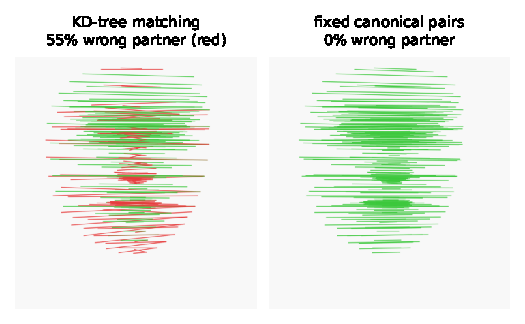
\includegraphics[width=\linewidth]{figures/correspondence.pdf}
\caption{\textbf{Correspondence matters.} Lines join each left-side vertex to its
partner for one test face (geometry only; see \cref{sec:ethics}). Left: baseline KD-tree
matching after reflection; red lines are matches that are not the anatomical twin.
Right: fixed pairs from the symmetric canonical model.}
\label{fig:corr}
\end{figure}

\subsection{The mirror test}
\label{sec:mirror}
We run the detector on $I$ and on its horizontal flip $I^{f}$. A point at $x'$ in $I^{f}$
lies at $W-x'$ in $I$ (MediaPipe uses continuous coordinates with pixel centres at
$i+\tfrac12$), and flipping swaps anatomical sides, so the vertex reported as $j$ in $I^{f}$
is vertex $\pi(j)$ of $I$:
\begin{equation}
U_{\pi(j)} = \bigl(W-L^{f}_{j,x},\;L^{f}_{j,y}\bigr).
\end{equation}
For an ideal detector $U\!=\!L$. We define the \emph{mirror inconsistency}
$\delta=\tfrac{1}{|\mathcal{I}|}\sum_{i\in\mathcal{I}}\|L_i-U_i\|/\mathrm{IOD}$ (and per region,
$\delta_r$), and measure asymmetry on the average $\bar L=\tfrac12(L+U)$.
\emph{Why:} the true asymmetry of a face does not change when the image is flipped, but
a detector's errors do not have to flip with it. The disagreement $\delta$ therefore
estimates landmark unreliability \emph{without ground truth}. MediaPipe exposes no
per-landmark confidence, so $\delta$ fills that gap. Averaging cancels any systematic
left/right bias of the detector, and $|A(L)-A(U)|$ is shown to the user as a stability
band. The cost is one extra detector pass (\runtime\,ms per image in total, including the
baseline's re-detection, on a 2-core 2.1\,GHz Xeon).

\subsection{Quality and pose gate}
\label{sec:gate}
The gate reads seven signals that the system can actually observe
(\cref{tab:thresholds}):
\textbf{face size} (IOD in pixels);
\textbf{sharpness}, $\log_{10}$ of the variance of the Laplacian~\cite{pertuz2013focus} on the face crop
resized to 256\,px width, so that it does not depend on face size;
\textbf{exposure}, the mean luma and the fraction of clipped pixels in the face crop;
\textbf{$|$yaw$|$, $|$pitch$|$} from the transformation matrix;
and the \textbf{mirror inconsistency} $\delta$.
In-plane roll is \emph{not} gated, because \cref{eq:axis} is invariant to it.
The worst signal decides accept / caution / reject, and every decision is shown with a
plain-language reason. A rejected image never shows a score unless the user explicitly
asks for it, and it is then labelled unreliable. In addition, a region whose
$\delta_r$ exceeds a training percentile is marked \emph{unreliable} and greyed out.

\textbf{Threshold policy} (fixed before looking at test results): pose and face-size limits
follow from the measurement's assumptions (yaw 10$^\circ$/20$^\circ$, pitch 15$^\circ$/25$^\circ$,
IOD 60/30\,px). Image-statistic limits are percentiles of the \emph{training} split: 2.5th
percentile of sharpness and of brightness for caution, and 90th/99th percentiles of
$\delta$. The test split is used only for evaluation.

\begin{table}[t]
\centering\footnotesize
\resizebox{\linewidth}{!}{\begin{tabular}{@{}llll@{}}
\toprule
Signal & caution & reject & source\\
\midrule
face size (IOD) & $<$ 60 px & $<$ 30 px & a priori\\
sharpness ($\log_{10}$ var. Lap.) & $<$ 1.4 & $<$ 0.756 & train pct.\\
mean luma (low) & $<$ 59.3 & $<$ 35 & train pct. / a priori\\
mean luma (high) & $>$ 164 & $>$ 225 & train pct. / a priori\\
clipped pixels & $>$ 0.364 & $>$ 0.6 & train pct. / a priori\\
$|$yaw$|$ & $>$ 10$^\circ$ & $>$ 20$^\circ$ & a priori\\
$|$pitch$|$ & $>$ 15$^\circ$ & $>$ 25$^\circ$ & a priori\\
mirror inconsistency $\delta$ & $>$ 0.0224 & $>$ 0.0489 & train pct.\\
per-region $\delta_r$ (validity) & \multicolumn{2}{l}{unreliable if $>$ 0.0444} & train pct.\\
\bottomrule
\end{tabular}
}
\caption{\textbf{Gate thresholds} (\texttt{configs/gate\_thresholds.json}).
``train pct.'': percentile of the \nTrainOk{} LFPW training faces.}
\label{tab:thresholds}
\end{table}

\subsection{Compared variants}
\label{sec:variants}
All variants use the \emph{same} detections of each image:
\textbf{M0} (baseline) is our re-implementation of~\cite{nashokan_facialasymmetry}: similarity
alignment of vertices 33/263 to fixed positions, re-detection, a vertical midline through
33/263, KD-tree reflected matching on all vertices, and the mean distance divided by face
width. That repository has no licence, so we re-implemented the method from its
description and code rather than copying it. Note that 33/263 are the \emph{outer} eye
corners, although the code comments call them inner corners.
\textbf{M1}: fixed 68-point pairs + fitted axis (\cref{sec:corr,sec:axis}).
\textbf{M2}: M1 + gate without $\delta$.
\textbf{M3} (full system): measurement on $\bar L$, gate with $\delta$, region validity.
